% Rapport Cavitation (M1, 2023-2024). Compiler dans outils/rapports/cavitation :
%   Rscript figures.R && xelatex cavitation && biber cavitation && xelatex cavitation
\documentclass[11pt,a4paper]{article}
\usepackage{../rapport-portfolio}
\definecolor{themehex}{HTML}{2F6E9E}\colorlet{theme}{themehex}
\addbibresource{references.bib}

\titrerapport{Variabilité génotypique et plasticité phénotypique de la résistance à la cavitation chez le peuplier}
\titrecourt{Cavitation chez le peuplier}
\soustitre{Effet de l'azote et de la sécheresse sur la P50 de quatre cultivars}
\auteurs{Jérémy Genty}
\cadre{Master 1 BICG · UE Génétique et amélioration des plantes · Université d'Orléans}
\annee{Compte rendu de travaux pratiques · 2023-2024}
\motcle{Écophysiologie forestière}
\visuel{%
\begin{tikzpicture}[x=44mm,y=0.95mm]
  \fill[theme!8,rounded corners=3mm] (-3.35,-14) rectangle (0.05,112);
  \foreach \y in {0,25,50,75,100} \draw[theme!25] (-3.2,\y) -- (-0.4,\y);
  \draw[theme!60,dashed,line width=0.6pt] (-3.2,50) -- (-0.4,50);
  \draw[line width=2.4pt,theme!45,domain=-3.2:-0.4,samples=80,smooth] plot (\x,{100/(1+exp(4*(\x+2.15)))});
  \draw[line width=2.4pt,theme,domain=-3.2:-0.4,samples=80,smooth] plot (\x,{100/(1+exp(4*(\x+1.83)))});
  \draw[theme,line width=0.8pt] (-1.83,-6) -- (-1.83,50); \fill[theme] (-1.83,50) circle (1.6mm);
  \draw[theme!45,line width=0.8pt] (-2.15,-6) -- (-2.15,50); \fill[theme!45] (-2.15,50) circle (1.6mm);
  \node[font=\small\bfseries,text=theme] at (-1.6,-10) {P50};
  \node[anchor=west,font=\small,text=gris] at (-3.25,104) {Perte de conductivité (\%)};
  \node[anchor=east,font=\small,text=gris] at (-0.45,-10) {Potentiel hydrique (MPa)};
\end{tikzpicture}}

\begin{document}
\pagedegarde

\enbref{Sous serre, l'apport optimal d'azote rend Skado et Koster plus vulnérables à l'embolie (P50 moins négative de 0,13 à 0,15~MPa). En pépinière, la fertilisation n'a plus d'effet net, mais les plants élevés sous sécheresse sont plus résistants chez les quatre cultivars, avec l'écart le plus fort chez Skado (-0,47~MPa) et Jean Pourpet (-0,34~MPa).}

\section{Introduction}
L'eau est une ressource limitante pour la croissance des plantes : elle intervient dans la photosynthèse, le port dressé et le transport des sèves. Le réchauffement climatique d'origine anthropique augmente la fréquence et l'intensité des sécheresses. Les arbres doivent y répondre rapidement, et cette réponse dépend de leur plasticité phénotypique.

Lors d'une sécheresse, la tension de la sève dans le xylème augmente jusqu'à rompre la colonne d'eau : des bulles d'air (embolies) bloquent alors les vaisseaux et la conductivité hydraulique chute \parencite{tyree1989}. La P50, potentiel hydrique pour lequel 50~\% de la conductivité est perdue, résume la résistance d'une espèce ou d'un génotype à l'embolie ; elle est étroitement liée au risque de dépérissement des forêts \parencite{choat2012}.

Le peuplier est un enjeu économique : en 2012, 60~\% du bois d'œuvre produit dans le Nord-Pas-de-Calais était du peuplier \parencite{zapater}. Le changement climatique impose de sélectionner des cultivars plus tolérants à la sécheresse. Ce travail compare donc la résistance à l'embolie de plusieurs génotypes de peuplier, et sa plasticité selon deux leviers contrôlables en culture : la fertilisation et l'irrigation.

\section{Matériel et méthodes}
\subsection{Matériel végétal}
Quatre cultivars ont été étudiés : Koster, hybride interspécifique \emph{Populus deltoides} × \emph{P. nigra} ; Skado, hybride \emph{P. trichocarpa} × \emph{P. maximowiczii} ; Dellinois, clone de \emph{P. deltoides} ; Jean Pourpet, clone de \emph{P. nigra}.

\subsection{Dispositif}
Deux expérimentations ont été menées (figure~\ref{fig:dispositif}) :
\begin{itemize}
\item \textbf{sous serre}, Skado et Koster, cinq copies clonales par génotype et par traitement, avec deux niveaux d'azote : apport basal (\og low-N \fg) et apport optimal (\og high-N \fg) ;
\item \textbf{en pépinière}, les quatre cultivars, trois copies clonales par génotype et par traitement (quatre pour Skado WF), avec trois traitements : irrigué sans fertilisation (WNF), irrigué et fertilisé avec un engrais NPK 21-6-8 (WF), non irrigué et non fertilisé (DNF).
\end{itemize}

\begin{figure}[ht]
\centering
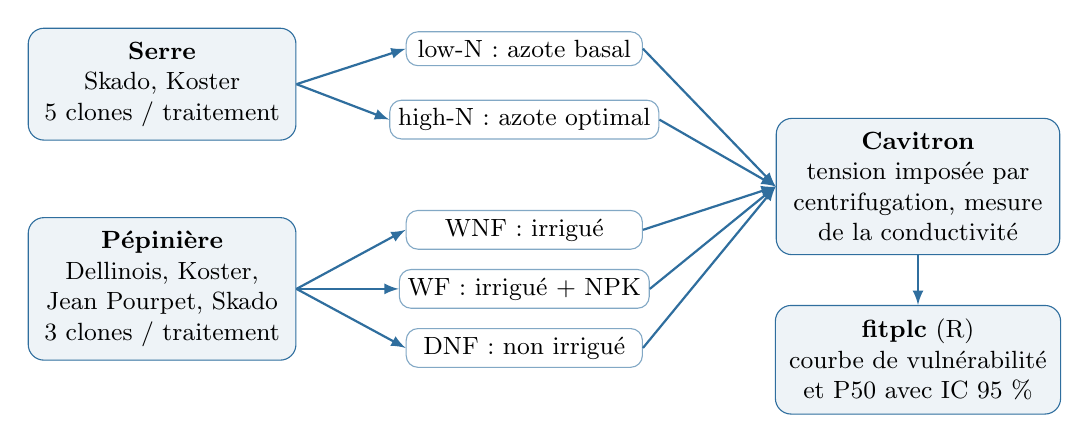
\begin{tikzpicture}[font=\small,
  boite/.style={draw=theme,fill=theme!8,rounded corners=2mm,align=center,inner sep=5pt},
  trt/.style={draw=theme!60,fill=white,rounded corners=1.5mm,align=center,inner sep=3pt,minimum width=30mm},
  fl/.style={-latex,theme,line width=0.8pt}]
  \node[boite,minimum width=34mm] (s) at (0,0) {\textbf{Serre}\\Skado, Koster\\5 clones / traitement};
  \node[trt] (s1) at (4.6,0.45) {low-N : azote basal};
  \node[trt] (s2) at (4.6,-0.45) {high-N : azote optimal};
  \node[boite,minimum width=34mm] (p) at (0,-2.6) {\textbf{Pépinière}\\Dellinois, Koster,\\Jean Pourpet, Skado\\3 clones / traitement};
  \node[trt] (p1) at (4.6,-1.85) {WNF : irrigué};
  \node[trt] (p2) at (4.6,-2.6) {WF : irrigué + NPK};
  \node[trt] (p3) at (4.6,-3.35) {DNF : non irrigué};
  \node[boite,minimum width=36mm] (c) at (9.6,-1.3) {\textbf{Cavitron}\\tension imposée par\\centrifugation, mesure\\de la conductivité};
  \node[boite,minimum width=36mm] (f) at (9.6,-3.5) {\textbf{fitplc} (R)\\courbe de vulnérabilité\\et P50 avec IC 95~\%};
  \foreach \n in {s1,s2} \draw[fl] (s.east) -- (\n.west);
  \foreach \n in {p1,p2,p3} \draw[fl] (p.east) -- (\n.west);
  \foreach \n in {s1,s2,p1,p2,p3} \draw[fl] (\n.east) -- (c.west);
  \draw[fl] (c) -- (f);
\end{tikzpicture}
\caption{Dispositif expérimental : deux essais (serre et pépinière), puis mesure de la vulnérabilité à l'embolie sur tiges au Cavitron.}
\label{fig:dispositif}
\end{figure}

\subsection{Mesures et analyse}
La vulnérabilité à l'embolie a été mesurée au Cavitron \parencite{cochard2005} : une tige est mise en rotation dans une centrifugeuse, ce qui impose au xylème une tension connue ; la conductivité hydraulique est mesurée à chaque palier de tension, de -0,5 à -3~MPa environ. On en déduit le pourcentage de perte de conductivité (PLC) en fonction du potentiel hydrique du xylème.

Pour chaque génotype et chaque traitement, une courbe de Weibull a été ajustée avec le package R \emph{fitplc} \parencite{duursma2017}, avec un effet aléatoire individu ; la P50 et son intervalle de confiance à 95~\% sont tirés de cet ajustement. Deux traitements sont jugés différents lorsque leurs intervalles de confiance ne se recouvrent pas, un critère conservateur.

\noterevision{Note de révision (2026) : la version de 2023 décrivait une mesure du potentiel hydrique du sol par sonde tensiométrique. Au Cavitron, c'est la tension du xylème qui est imposée par la centrifugation ; le texte est corrigé en ce sens. Les P50 ont été recalculées à partir des données brutes du TP.}

\section{Résultats}
\subsection{Serre : effet de l'azote}
Chez Skado comme chez Koster, la P50 est moins négative avec un apport optimal d'azote (figure~\ref{fig:serre}, tableau~\ref{tab:p50}) : -1,22~MPa contre -1,37~MPa pour Skado, -1,18~MPa contre -1,31~MPa pour Koster. Les intervalles de confiance ne se recouvrent pas : l'apport d'azote rend ces deux génotypes plus vulnérables à l'embolie.

\begin{figure}[ht]
\centering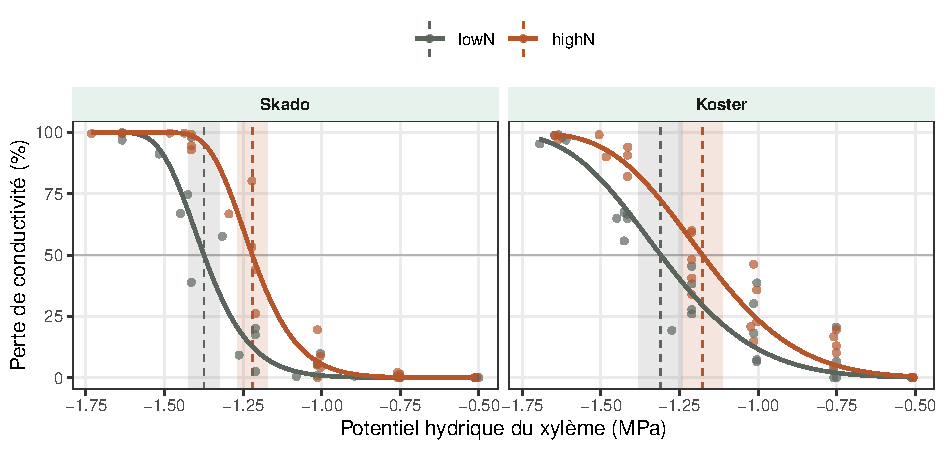
\includegraphics[width=\linewidth]{figures/fig_serre.pdf}
\caption{Courbes de vulnérabilité sous serre selon l'apport d'azote. Trait plein : ajustement de Weibull ; tirets verticaux : P50 ; bandes : intervalle de confiance à 95~\%.}
\label{fig:serre}
\end{figure}

\subsection{Pépinière : effet de la fertilisation}
En pépinière, les intervalles de confiance des P50 avec et sans fertilisation se recouvrent pour les quatre cultivars (figure~\ref{fig:ferti}). Les P50 sont aussi nettement plus négatives que sous serre, entre -1,83 et -2,14~MPa : les plants élevés en extérieur sont plus résistants.

\begin{figure}[ht]
\centering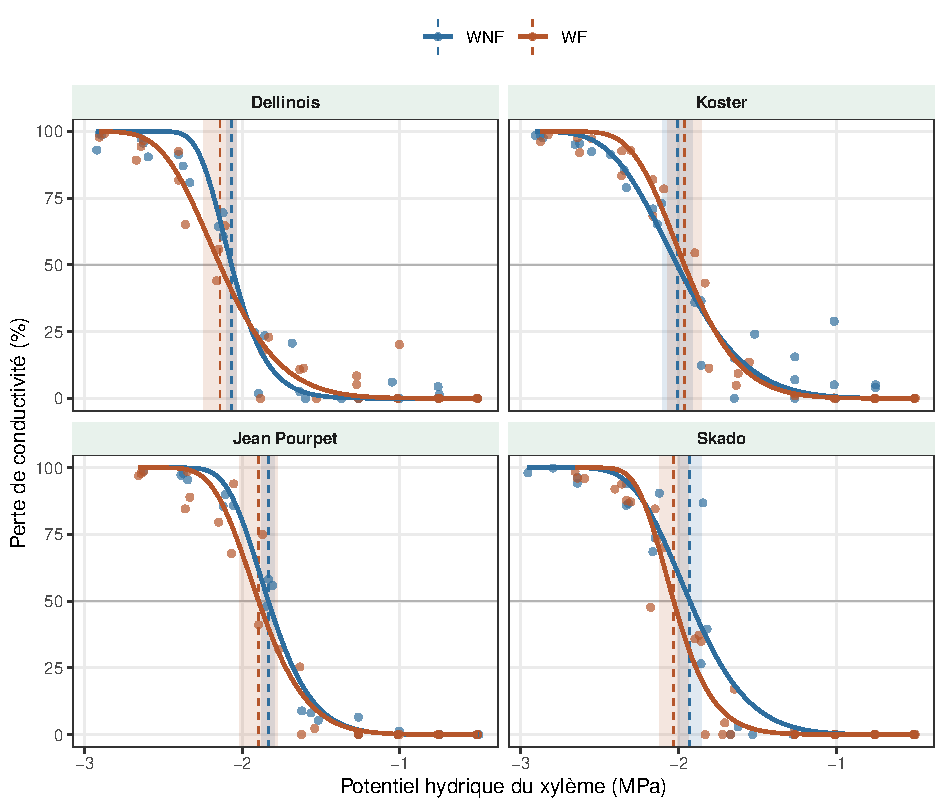
\includegraphics[width=0.8\linewidth]{figures/fig_fertilisation.pdf}
\caption{Courbes de vulnérabilité en pépinière : irrigué sans fertilisation (WNF) et irrigué fertilisé (WF).}
\label{fig:ferti}
\end{figure}

\subsection{Pépinière : effet de la sécheresse}
Les plants élevés sans irrigation (DNF) ont une P50 plus négative que les plants irrigués (WNF) chez les quatre cultivars, sans recouvrement des intervalles de confiance (figure~\ref{fig:irrig}). L'écart est faible chez Dellinois (-0,13~MPa) et Koster (-0,15~MPa), plus marqué chez Jean Pourpet (-0,34~MPa) et surtout Skado (-0,47~MPa).

\begin{figure}[ht]
\centering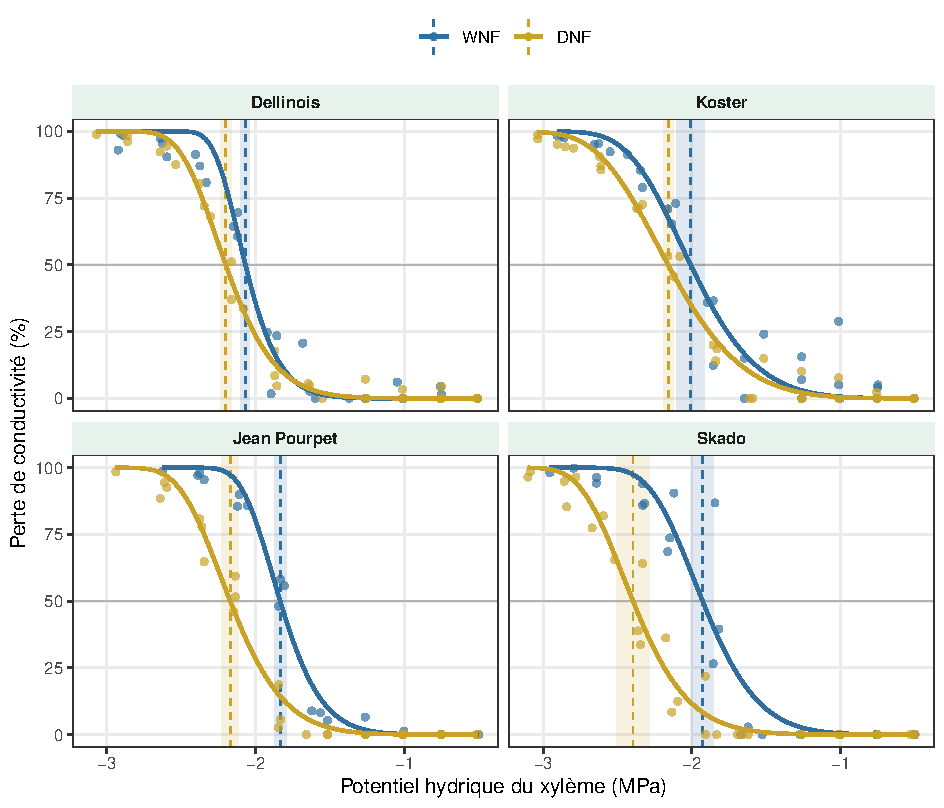
\includegraphics[width=0.8\linewidth]{figures/fig_irrigation.pdf}
\caption{Courbes de vulnérabilité en pépinière : irrigué (WNF) et non irrigué (DNF).}
\label{fig:irrig}
\end{figure}

\begin{table}[ht]
\centering\small
\caption{P50 (MPa) et intervalle de confiance à 95~\% par génotype et par traitement (fitplc, effet aléatoire individu).}
\label{tab:p50}
\begin{tabular}{@{}llrr@{}}
\toprule\entete
Essai & Génotype & \multicolumn{1}{c}{Traitement : P50 [IC 95~\%]} & \multicolumn{1}{c}{Traitement : P50 [IC 95~\%]}\\
\midrule
Serre & Skado & low-N : -1,37 [-1,43 ; -1,32] & high-N : -1,22 [-1,27 ; -1,17]\\
 & Koster & low-N : -1,31 [-1,38 ; -1,24] & high-N : -1,18 [-1,24 ; -1,11]\\
\midrule
Pépinière & Dellinois & WNF : -2,07 [-2,10 ; -2,04] & WF : -2,14 [-2,24 ; -2,04]\\
 & Koster & WNF : -2,01 [-2,10 ; -1,91] & WF : -1,96 [-2,07 ; -1,86]\\
 & Jean Pourpet & WNF : -1,83 [-1,88 ; -1,79] & WF : -1,90 [-2,02 ; -1,78]\\
 & Skado & WNF : -1,93 [-2,00 ; -1,85] & WF : -2,03 [-2,12 ; -1,94]\\
\midrule
Pépinière & Dellinois & & DNF : -2,20 [-2,24 ; -2,16]\\
 & Koster & & DNF : -2,16 [-2,19 ; -2,13]\\
 & Jean Pourpet & & DNF : -2,17 [-2,23 ; -2,11]\\
 & Skado & & DNF : -2,40 [-2,51 ; -2,28]\\
\bottomrule
\end{tabular}
\end{table}

\section{Discussion}
L'effet de l'azote observé sous serre va dans le sens de la littérature : chez le peuplier hybride, la fertilisation azotée produit des vaisseaux plus larges, plus efficaces mais plus vulnérables à l'embolie \parencite{plavcova2012}. Cet effet disparaît en pépinière, où d'autres facteurs (climat, sol, hétérogénéité entre plants) pèsent davantage, et où l'engrais NPK n'est pas strictement comparable à l'apport d'azote de la serre.

La sécheresse de croissance, au contraire, renforce la résistance à l'embolie chez les quatre cultivars : c'est une acclimatation déjà décrite chez le peuplier \parencite{awad2010}. Son ampleur varie selon le génotype : Skado et Jean Pourpet sont les plus plastiques, Dellinois et Koster les moins.

Ces résultats reposent sur peu d'individus (trois par traitement en pépinière) et sur un seul site : l'effet aléatoire individu est d'ailleurs quasi nul dans plusieurs ajustements, signe que la variabilité entre plants est mal estimée. Le critère de non-recouvrement des intervalles reste prudent, mais un test formel et davantage de répétitions seraient nécessaires.

\noterevision{Note de révision (2026) : la version de 2023 ne retenait un effet de la sécheresse que pour Jean Pourpet. Le recalcul des P50 avec le même modèle montre un effet chez les quatre cultivars ; la discussion est corrigée en conséquence.}

\section{Conclusion et perspectives}
L'azote augmente la vulnérabilité à l'embolie quand le milieu est contrôlé, et une croissance sous contrainte hydrique l'abaisse chez tous les cultivars testés. Pour la populiculture, cela suggère d'éviter une fertilisation azotée forte là où les sécheresses sont fréquentes, et de privilégier les cultivars les plus plastiques, ici Skado et Jean Pourpet. Il resterait à vérifier que ce gain de résistance ne se paie pas en croissance, et à croiser sécheresse et fertilisation dans un même essai.

\pagebiblio
\end{document}
